% This work is licensed under the Creative Commons Attribution-NonCommercial 4.0 International License.
% To view a copy of this license, visit http://creativecommons.org/licenses/by-nc/4.0/
% or send a letter to Creative Commons, PO Box 1866, Mountain View, CA 94042, USA.

% !TEX TS-program = xelatex

\documentclass[../Main/chem331-notes.tex]{subfiles}
\begin{document}

\setcounter{section}{12}

\section{The hydrogen atom}
\subsection{The classical Coulomb potential}
In our treatment of the hydrogen atom we will start by assuming that the proton is fixed in space and we will only consider the wave function of the electron. The potential experienced by the electron orbiting around the proton is then
\begin{equation}
V(x,y,z) = - \frac{1}{4 \pi \epsilon_0} \frac{e^2}{r}
\end{equation}
where $\epsilon_0$ is the vacuum permittivity.
For convenience we will switch right away to atomic units, for which the term
\begin{equation}
\frac{e^2}{4 \pi \epsilon_0} = 1 \quad \text{(in atomic units)}.
\end{equation}
This leaves us with the much simpler form for the potential
\begin{equation}
V(x,y,z) = - \frac{1}{r}.
\end{equation}

\subsection{The Hamiltonian}
The Hamiltonian of the hydrogen atom in Cartesian coordinates is given by
\begin{equation}
\hat{H} = -\frac{1}{2} \nabla^2 - \frac{1}{r} = -\frac{1}{2} \left(\frac{\partial^2}{\partial x^2} + \frac{\partial^2}{\partial y^2} + \frac{\partial^2}{\partial z^2} \right) - \frac{1}{\sqrt{x^2 + y^2 + z^2}},
\end{equation}
and as we have seen before, it is more convenient to write it in spherical coordinates as
\begin{equation}
\hat{H} =  -\frac{1}{2} \left[ \frac{1}{r^2} \frac{\partial}{\partial r} \left( r^2 \frac{\partial }{\partial r} \right)
+ \frac{1}{r^2 \sin \theta} \frac{\partial}{\partial \theta} \left( \sin\theta \frac{\partial }{\partial \theta} \right)
+ \frac{1}{r^2 \sin^2 \theta} \frac{\partial^2}{\partial \phi^2} \right]  - \frac{1}{r}.
\end{equation}
Part of this Hamiltonian are related to angular momentum.
In spherical coordinates the angular momentum squared operator ($\hat{L}^2$) is given by the following equation (note that there is an imiplicit $\hbar^2$ factor that  goes away when we write $\hat{L}^2$ in atomic units)
\begin{equation}
\hat{L}^2 = - \left[\frac{1}{ \sin \theta} \frac{\partial}{\partial \theta} \left( \sin\theta \frac{\partial }{\partial \theta} \right)
+ \frac{1}{ \sin^2 \theta} \frac{\partial^2}{\partial \phi^2} \right].
\end{equation}
Using the definition of $\hat{L}^2$ in spherical coordinates it is possible to write the Hamiltonian in a more compact way
\begin{equation}
\hat{H} =  -\frac{1}{2} \left[ \frac{1}{r^2} \frac{\partial}{\partial r} \left( r^2 \frac{\partial }{\partial r} \right)
- \frac{\hat{L}^2}{r^2}  \right]  - \frac{1}{r}.
\end{equation}
To find the eigenvalues and eigenfunctions of $\hat{H}$ we attempt to write the solution in a factorized form
\begin{equation}
\psi(r,\theta,\phi) = R(r) Y_l^{m_l}(\theta,\phi),
\end{equation}
where $R(r)$ is the \textbf{radial wave function} and $Y_l^{m_l}(\theta,\phi)$ is a spherical harmonic.\mnote{To follow the conventional scheme to label the solution of the hydrogen atom here we use the symbol $m_l$ instead of $m$.}
If we plug this guess into the Schr\"{o}dinger equation we get
\begin{equation}
\begin{split}
\hat{H}\psi(r,\theta,\phi) & =  -\frac{1}{2} \left[ \frac{1}{r^2} \frac{\partial}{\partial r} \left( r^2 \frac{\partial }{\partial r} \right)
- \frac{\hat{L}^2}{r^2}  \right]R(r) Y_l^{m_l}(\theta,\phi)  - \frac{R(r) Y_l^{m_l}(\theta,\phi)}{r} \\
& = -\frac{1}{2} Y_l^{m_l}(\theta,\phi) \left[ \frac{1}{r^2} \frac{\partial}{\partial r} \left( r^2 \frac{\partial  }{\partial r} \right)
- \frac{l(l+1)}{r^2}  \right] R(r)  - \frac{R(r) Y_l^{m_l}(\theta,\phi)}{r} \\
& = E R(r) Y_l^{m_l}(\theta,\phi).
\end{split}
\end{equation}
Note that all the operator components that act on $\theta$ and $\phi$ are contained in the $\hat{L}^2$ operator. Since $Y_l^{m_l}(\theta,\phi)$ is an eigenfunction of $\hat{L}^2$, in the second step we were able to replace $\hat{L}^2Y_l^{m_l}(\theta,\phi)$ with $l(l+1)Y_l^{m_l}(\theta,\phi)$.
Since $Y_l^{m_l}(\theta,\phi)$ multiplies both sides of this equation, we can remove this factor and obtain an equation for the radial wave function alone
\begin{equation}
\Big[\underbrace{
 -\frac{1}{2r^2} \frac{\partial}{\partial r} \left( r^2 \frac{\partial  }{\partial r} \right)
 }_{\text{kinetic}}
+ \underbrace{
\frac{l(l+1)}{2r^2} - \frac{1}{r}
}_{\text{potential}}
\Big] R(r) = E R(r).
\end{equation}
We can identify two contributions to this equation. The first one contains derivatives with respect to $r$ and can be associated with the kinetic energy.
The second term
 \begin{equation}
V_l(r) = \frac{l(l+1)}{2r^2} - \frac{1}{r},
\end{equation}
can be considered an effective Coulomb potential. It contains the correct $- r^{-1}$ term that we expect from the classical Coulomb potential plus a term proportional to $r^{-2}$.
The latter, is due to angular momentum and counters the effect of Coulomb attraction.
Since the effective potential depends on $l$, we have to solve a different radial Schr\"{o}dinger equation for each value of $l$.

Note that the radial equation is sometimes expressed as a function of the variable
\begin{equation}
\rho = 2r,
\end{equation}
so that the left hand side can be written as\mnote{
$\frac{\partial}{\partial r} = \frac{\partial\rho}{\partial r} \frac{\partial}{\partial \rho} = \frac{2}{n} \frac{\partial}{\partial \rho}$.
}
\begin{equation}
-\frac{1}{2r^2} \frac{\partial}{\partial r} \left( r^2 \frac{\partial  }{\partial r} \right) + \frac{l(l+1)}{2r^2} - \frac{1}{r}
= -2 \frac{\partial^2}{\partial \rho^2}
-\frac{4}{\rho} \frac{\partial}{\partial \rho} + 2\frac{l(l+1)}{\rho^2} - \frac{2}{\rho},
\end{equation}
and can be used to write the Schr\"{o}dinger equation as
\begin{equation}
\left[
-\frac{\partial^2 }{\partial \rho^2}
-\frac{2}{\rho}\frac{\partial }{\partial \rho}
-\frac{1}{\rho} + \frac{l(l+1)}{\rho^2} \right] R(\rho) = E' R(\rho),
\end{equation}
where the energy $E' = E / 2$.

The solution of the radial equation is quite involved and we will jump directly to the solution. The eigenvalues ($E_n$ of the radial equation are given by
\begin{iequation}
E_n = - \frac{1}{2 n^2}  \, E_\mathrm{h},
\end{iequation}
with the energy being expressed in Hartree (symbol $E_\mathrm{h}$), the unit of measure of energy in atomic units. (1 $E_\mathrm{h}$ = 627.51 kcal mol$^{-1}$ = 27.211 eV).
The same expression in SI units is
\begin{equation}
E_n = - \frac{m_e e^4}{32 \pi^2\epsilon_0^2 \hbar^2 n^2} \, \mathrm{J}.
\end{equation}

The corresponding eigenfunctions are
\begin{equation}
R_{n,l}(\rho) = \sqrt{\left(\frac{2}{n} \right)^{3} \frac{ (n-l-1)! }{ 2n (n+l)!} }\left(\frac{\rho}{n}\right)^l e^{-\rho/2n} L_{n-l-1}^{2l+1}(\rho/n),
\end{equation}
%\begin{equation}
%R_{n,l}(r) = N_{n,l} \left(\frac{\rho}{n}\right)^l L_{n,l}(\rho) e^{-\rho/2n},
%\end{equation}
where $n$ is called the \textbf{principal quantum number} and can take the following values
\begin{equation}
n = 1, 2, 3, \ldots
\end{equation}
The quantity $L_{n+l}^{2l+1}(x)$ indicates \textbf{associated Laguerre polynomials}.
Converting from $\rho$ to $r$ we can write the radial equation in an equivalent way as
\begin{equation}
R_{n,l}(r) = \sqrt{\frac{ (n-l-1)! }{ 2n (n+l)!} } \left(\frac{2}{n} \right)^{l + 3/2} r^l e^{-r/n} L_{n-l-1}^{2l+1}(2r/n).
\end{equation}
The first few associated Laguerre polynomials are
\begin{equation}
\begin{split}
L_0^\alpha(x) & = 1 \\
L_1^\alpha(x) & = \alpha - x + 1 \\
L_2^\alpha(x) & = \frac{x^2}{2} - (\alpha + 2) x + \frac{(\alpha + 2)(\alpha + 1)}{2}.
\end{split}
\end{equation}

From the general solution for the hydrogen atom wave function we can get the ground state radial wave function ($n = 1$, $l = 0$)
\begin{equation}
R_{1,0}(r) =
\sqrt{\frac{ (0)! }{ 2 (1)!} } \left(\frac{2}{1} \right)^{3/2} r^0 e^{-r} \underbrace{L_{0}^{1}(2r)}_{1}
= \sqrt{\frac{1}{ 2} } \left(2\right)^{ 3/2} e^{-r} = 2 e^{-r}.
\end{equation}

The first few radial wave functions for larger values of $n$ and $l$ are
\begin{equation}
\begin{split}
R_{1,0}(r) & = 2 e^{-r}, \\
R_{2,0}(r) & =\frac{2 - r}{2 \sqrt{2}} e^{-r/2}, \\
R_{2,1}(r) & =\frac{r}{2 \sqrt{6}} e^{-r/2}, \\
R_{3,0}(r) & =\frac{27 - 18 r + 2 r^2}{81 \sqrt{3}} e^{-r/3}.
\end{split}
\end{equation}

\subsection{Quantum numbers and degeneracy}
Combining the results of the previous section we can write the wave function of the hydrogen atom in terms of three quantum numbers
\begin{equation}
\psi_{nlm_l}(r,\theta,\phi) = R_{nl}(r) Y_l^{m_l}(\theta,\phi),
\end{equation}
The principal quantum number $n$ is a positive integer and is connected to the total energy of a quantum state. 
In addition to the principal quantum number $n$ the wave function depends on the \textbf{angular momentum quantum number} $l$.  The allowed values of this quantum number are
\begin{iequation}
l = 0, 1, \ldots, n-1,
\end{iequation}
and it determines the total angular momentum squared of the hydrogen atom since
\begin{equation}
\langle \hat{L}^2 \rangle = \hbar^2 l(l + 1).
\end{equation}
In the convention used to label states of the hydrogen atom we assign symbols to different values of $l$. For $l = 0$ we label the state as $s$, $l = 1$ corresponds to $p$, $l= 2$ to $d$, and $l = 3$ to $f$. After $l=3$ we use letters in alphabetical order ($g$, $h$, $i$,\ldots).
The \textbf{magnetic quantum number} $m_l$ can take any of the following values
\begin{iequation}
m = 0, \pm 1, \pm 2,  \ldots, l.
\end{iequation}
For each value of $l$ there are $2l +1$ possible values of $m_l$. 
The magnetic quantum number is related to the projection of angular momentum on the $z$ axis
\begin{equation}
\langle \hat{L}_z \rangle = \hbar m_l.
\end{equation}

The states of the hydrogen atom are usually written as $nl$, using the corresponding symbol for $l$.
For example, the ground state ($n=1$, $l=0$) is designated 1s. The state ($n=2$, $l=0$) is indicates with 2s. The state ($n=2$, $l=1$) corresponds to 2p and ($n=3$, $l=2$) to 3d.
In addition, we may also label individual orbitals by adding a subscript that indicates the value of $m_l$.
For example, the 2p level is comprised of the orbitals 2p$_{-1}$, 2p$_{0}$, and 2p$_{1}$. Another example is the state 3d$_{-1}$, which corresponds to $n = 3$, $l = 2$, and $m_l = -1$.

Since the energy depends only on the quantum number $n$, states with different values of $l$ and $m_l$ but same $n$ will be degenerate.
For each value of $l$ there are $2l +1$ possible values of $m_l$. If we sum up all the possible states for a fixed $l$ we have that the total number of states for a given $n$ is equal to\mnote{Here we use the equation for the sum of the first $n$ integers, $\sum_{k = 1}^{n} k = 1+2+\ldots + n = n (n+1) / 2 $.}
\begin{equation}
\text{Degeneracy of level } n = \sum_{l = 0}^{n-1} (2l +1) = 2 \sum_{l = 0}^{n-1} l + \sum_{l = 0}^{n-1} 1
= 2 \frac{(n - 1) n}{2} + n = n^2.
\end{equation}

\subsection{Eigenfunctions of the hydrogen atom}
The solution to the hydrogen atom Schr\"{o}dinger equation are expressed in terms of spherical harmonics. These functions are complex (due to the $e^{i m_l \phi}$ term) and are difficult to use and reason about in the context of molecular orbital theory.
For these reasons, it is convenient to convert atomic orbitals expressed using spherical harmonics into what are called Cartesian spherical harmonics.
The wave function for the ground state of hydrogen is real, this is what we call the 1s orbital
\begin{equation}
\mathrm{1s} = \psi_{1,0,0}(r,\theta,\phi) = R_{1,0}(r) Y_0^0(\theta,\phi) = 2 e^{-r} \frac{1}{\sqrt{4\pi}} = \frac{1}{\sqrt{\pi}} e^{-r}.
\end{equation}
Of the 2p orbitals, 2p$_{1}$ and 2p$_{-1}$ are instead complex
\begin{align}
\mathrm{2p}_{1} &= \psi_{2,1,1}(r,\theta,\phi) = R_{2,1}(r) Y_1^1(\theta,\phi) =
\frac{1}{8\sqrt{\pi}}   r e^{-r/2} \sin \theta e^{i\phi}, \\
\mathrm{2p}_{-1} &= \psi_{2,1,-1}(r,\theta,\phi) = R_{2,1}(r) Y_1^{-1}(\theta,\phi) =
\frac{1}{8\sqrt{\pi}}   r e^{-r/2} \sin \theta e^{-i\phi}, \\
\mathrm{2p}_{0} &= \psi_{2,1,0}(r,\theta,\phi) = R_{2,1}(r) Y_1^{0}(\theta,\phi) =
\frac{1}{4\sqrt{2 \pi}}   r e^{-r/2} \cos \theta.
\end{align}
To convert the 2p$_{1}$ and 2p$_{-1}$ orbitals to Cartesian harmonics we take linear combinations of the spherical harmonics. Taking the plus combination we get
\begin{equation}
\begin{split}
S_1^x = \frac{1}{\sqrt{2}} \left[ Y_1^1(\theta,\phi) + Y_1^{-1}(\theta,\phi) \right]
& = \frac{1}{\sqrt{2}} \left( \frac{3}{8\pi} \right)^{1/2} \sin \theta \left( e^{i\phi} + e^{-i\phi} \right) \\
& = \sqrt{2} \left( \frac{3}{8\pi} \right)^{1/2} \sin \theta \cos \phi \\
& = \left( \frac{3}{4\pi} \right)^{1/2} \frac{x}{r},
\end{split}
\end{equation}
while the minus combination gives
\begin{equation}
\begin{split}
S_1^y = \frac{1}{i\sqrt{2}} \left[ Y_1^1(\theta,\phi) - Y_1^{-1}(\theta,\phi) \right]
& = \frac{1}{i\sqrt{2}} \left( \frac{3}{8\pi} \right)^{1/2} \sin \theta \left( e^{i\phi} - e^{-i\phi} \right) \\
& = \sqrt{2} \left( \frac{3}{8\pi} \right)^{1/2} \sin \theta \sin \phi \\
& = \left( \frac{3}{4\pi} \right)^{1/2} \frac{y}{r}.
\end{split}
\end{equation}
If we compare these new  Cartesian harmonics $S_1^x$ and $S_1^y$ to the $Y_1^0$ harmonic
\begin{equation}
Y_1^0(\theta,\phi) = \left( \frac{3}{4\pi} \right)^{1/2} \cos \theta = \left( \frac{3}{4\pi} \right)^{1/2} \frac{z}{r},
\end{equation}
we notice that they are nothing else than $Y_1^0$ but oriented in the $x$ or $y$ direction. We can also identify the spherical harmonic $Y_1^0$ with the Cartesian harmonic in the $z$ direction, $Y_1^0 = S_1^z$.
From Cartesian harmonics we can build Cartesian atomic orbitals
\begin{align}
\mathrm{2p}_{x} &= R_{2,1}(r) S_1^x(\theta,\phi) =
\frac{1}{4\sqrt{2 \pi}} e^{-r/2} x, \\
\mathrm{2p}_{y} &= R_{2,1}(r) S_1^{y}(\theta,\phi) =
\frac{1}{4\sqrt{2 \pi}} e^{-r/2} y, \\
\mathrm{2p}_{z} &= R_{2,1}(r) S_1^{z}(\theta,\phi) =
\frac{1}{4\sqrt{2 \pi}} e^{-r/2} z.
\end{align}
These are shown in Fig.~\ref{fig:hydrogenatom:cartesianorbitals}.

\begin{figure}[t!]
   \centering
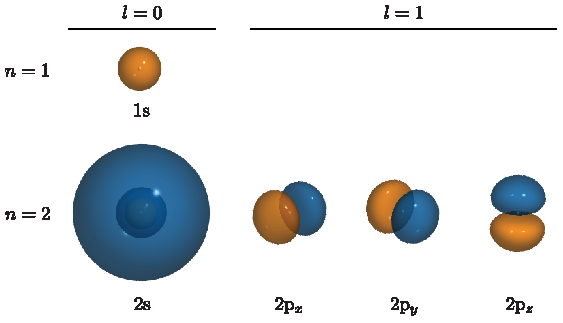
\includegraphics[width=3.75in]{../Figures/HydrogenAtom/CartesianOrbitals.pdf}
\captionof{figure}{Hydrogen atom wave functions for $n = 1$ and $n = 2$. The 2p orbitals are represented using Cartesian harmonics.}
\label{fig:hydrogenatom:cartesianorbitals}
\end{figure}

This transformation can be performed also on d and higher angular momentum functions. In the case of 3d orbitals, the orbitals expressed using spherical harmonics are 3d$_{2}$, 3d$_{1}$, 3d$_{0}$, 3d$_{-1}$, and 3d$_{-2}$.
The resulting orbitals are shown in Fig.~\ref{fig:hydrogenatom:dorbitals} and are usually labeled as 3d$_{z^2}$, 3d$_{xy}$, 3d$_{yz}$, 3d$_{xz}$, and 3d$_{x^2-y^2}$.
Note that the 3d$_{z^2}$ orbital is sometimes referred to as 3d$_{3z^2 - r^2}$ or 3d$_{2z^2 - x^2 - y^2}$.
\begin{figure}[b!]
   \centering
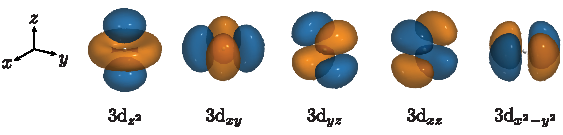
\includegraphics[width=3.75in]{../Figures/HydrogenAtom/DOrbitals.pdf}
\captionof{figure}{3d shell of the hydrogen atom ($n = 3$, $l = 2$). The 3d orbitals are represented using Cartesian harmonics.}
\label{fig:hydrogenatom:dorbitals}
\end{figure}

%For a fixed value of $l$, for example the $p$ series ($l = 1$), we have that the orbitals become more diffuse as $n$ increases.
%The number of nodes also increases. For $s$ type orbitals with a given $n$, we have $n-1$ radial nodes. For $p$ orbitals, there are $n -2$ for a orbitals with quantum number $n$.

%It is convenient to transform the hydrogen atom from the definition given in terms of spherical harmonics to one in terms of real functions.

\subsection{Where is the electron?}
In this section we analyze the ground state wave function for the hydrogen atom.
The ground state wave function is given by
\begin{equation}
\psi_{1,0,0}(r,\theta,\phi) = \frac{1}{\sqrt{\pi}} e^{-r}.
\end{equation}
This function has a maximum for $r = 0$. So the position $r = 0$ is the point in space where the probability of finding the electron is highest.

\marginpar{
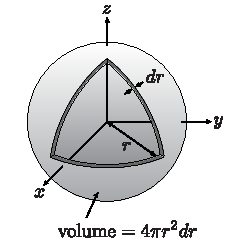
\includegraphics[width=1.5in]{../Figures/HydrogenAtom/SphericalShell.pdf}
\captionof{figure}{Radial shell of radius $r$ and thickness $dr$.}
\label{fig:hydrogenatom:sphericalshell}
}

We can also analyze this wave function from the point of view of the \textbf{radial probability distribution},
that is, we can ask, what is the probability that the electron lies within a spherical shell with radius between $r$ and $r + dr$, as shown in Fig.~\ref{fig:hydrogenatom:sphericalshell}.
The spherical shell has a volume that is proportional to $r^2$ and we will see that this factor will enter in the radial probability distribution function. This factor accounts for the fact that as the radius grows we are summing the probability in larger slices of space.
To identify the radial probability distribution we write the normalization condition for a generic wave function of the hydrogen atom as
\begin{equation}
\int_{0}^{\infty} dr
\int_{0}^{\pi} d\theta
\int_{0}^{2\pi} d\phi \,r^2 \sin \theta |R_{n,l}(r) Y_l^{m_l}(\theta,\phi)|^2
= \int_{0}^{\infty} \,r^2 |R_{n,l}(r)|^2 dr = 1,
\end{equation}
where in the second step we used the normalization condition for the spherical harmonics.
The second integral suggests that we identify the quantity radial probability distribution, $P_{n,l}(r)$, as the quantity
\begin{equation}
P_{n,l}(r) = |R_{n,l}(r)|^2 r^2.
\end{equation}
For the ground state of the hydrogen atom we find that the radial probability distribution is equal to
\begin{equation}
P_{1,0}(r) =4 e^{-2r} r^2.
\end{equation}
To find the maximum of this function we take the first derivative and set it to zero
\begin{equation}
\frac{d P_{1,0}(r)}{dr} =4 \frac{d e^{-2r} r^2}{dr} = -8 e^{-2r} r^2 + 8 e^{-2r} r = 8 e^{-2r} r (1 - r) = 0.
\end{equation}
This condition is satisfied for $r = 0$ and $r = 1$. The former is a minimum while the latter is a maximum.
So the maximum of the radial probability distribution is at $r=1$, and we can interpret this result as saying that  the most probable radius for the electron is 1 $a_0$ (1 bohr). This agrees with the result from the Bohr model.

Alternatively, we can also ask what is the average radius. This quantity can be obtained by computing the expectation value of the quantity $r$
\begin{equation}
\langle r \rangle = \int_{0}^{\infty} dr
\int_{0}^{\pi} d\theta
\int_{0}^{2\pi} d\phi \,r^3 \sin \theta |R_{n,l}(r) Y_l^{m_l}(\theta,\phi)|^2
= \int_{0}^{\infty} \,r^3 |R_{n,l}(r)|^2 dr.
\end{equation}
For the ground state of the hydrogen atom we have to compute the integral
\begin{equation}
\langle r \rangle = \int_{0}^{\infty} \, 4 e^{-2r} r^3 \, dr = 4 \int_{0}^{\infty} \, e^{-2r} r^3 \, dr,
\end{equation}
which can be evaluated using the integral identity
\begin{equation}
\int_{0}^{\infty} x^n e^{-ax}  \, dr = \frac{n!}{a^{n+1}}.
\end{equation}
If we plug in this integral we get
\begin{equation}
\langle r \rangle_{1\mathrm{s}} = 4 \int_{0}^{\infty} \, e^{-2r} r^3 \, dr = 4 \frac{3!}{2^4} = 4 \frac{2 \cdot 3}{16} = \frac{3}{2} a_0.
\end{equation}

To summarize, for the ground state of the hydrogen atom we have that
\begin{ibox}
\begin{myitems}
\item There is a finite probability of finding the electron at the nucleus. The point in space with the \textbf{highest probability of finding the electron} is the nucleus (maximum of $|\psi|^2$).
\item The maximum of the radial probability distribution tells us the \textbf{most likely radius of the electron}  (maximum of $|\psi|^2 r^2$). For the ground state the most likely radius is 1 $a_0$, a value that is consistent with Bohr's model.
\item The \textbf{average radius} of the electron is $\frac{3}{2} a_0$ ($\langle r \rangle_{1\mathrm{s}}$). This is larger than the most likely radius.
\end{myitems}
\end{ibox}

\marginpar{
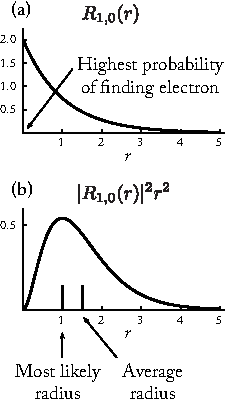
\includegraphics[width=1.5in]{../Figures/HydrogenAtom/WhereIsElectron.pdf}
\captionof{figure}{Ground state wave function of the hydrogen atom. (a) Radial wave function and (b) radial probability distribution.}
\label{fig:hydrogenatom:whereiselectron}
}

\subsection{Angular momentum and magnetic moment}
From classical electromagnetism we know that a magnetic dipole ($\boldsymbol{\mu}$) in a magnetic field ($\mathbf{B}$) has an energy equal to
\begin{equation}
V = - \boldsymbol{\mu} \cdot \mathbf{B}.
\end{equation}
As the electron orbits around the nucleus, it produces a magnetic moment that is proportional to its total angular momentum.
To see this recall that the modulus of the momentum $\mu = |\boldsymbol{\mu}|$ is given by Ampere's law: $\mu = I S$, where $I$ is the current generated by a charged particle moving around a circle of area $S$.
Let us consider a particle with charge $q$ and mass $m$ moving around a circle of radius $r$ perpendicular to the $z$ axis and with angular velocity $\omega$.
The current is given by the amount of charge ($q$) divided by the time it takes to go around the circle in a unit of time. If we defined the time it takes to go around the circle as $T = \frac{2 \pi r }{v} =\frac{2 \pi }{\omega}$ we can write the current as
\begin{equation}
I = \frac{q}{T} = \frac{q \omega}{2 \pi}.
\end{equation}
Then the modulus of the magnetic moment is given by
\begin{equation}
\mu = I S = \frac{q \omega}{2 \pi} \pi r^2 = \frac{q \omega r^2}{2} = \frac{q}{2m} L.
\end{equation}
where we have used the fact that the area is equal to $S = \pi r^2$ and that for a particle moving on a ring the modulus of the angular momentum is equal to $L = r mv = m r^2 \omega$.
Now we can attempt to quantize this expression by replacing all quantities with operators
\begin{equation}
\hat{\boldsymbol{\mu}} =  \frac{q}{2m} \hat{\mathbf{L}}.
\end{equation}

%For a hydrogen atom 
%\begin{equation}
%|L| = \hbar \sqrt{l (l + 1)},
%\end{equation}
%and
%\begin{equation}
%\mu = -\frac{\hbar e}{2m_e}  \sqrt{l (l + 1)} = - \beta_\mathrm{B} \hbar \sqrt{l (l + 1)},
%\end{equation}
%where the constant $\beta_\mathrm{B} = \frac{\hbar e}{2m_e}$ is called the Bohr magneton.

Now we can study what happens when we place a hydrogen atom in a magnetic field. If the magnetic field points towards the $z$ axis, the potential due to the field is given by
\begin{equation}
V = - \hat{\boldsymbol{\mu}} \cdot \mathbf{B} = - \mu_z B_z = \frac{\beta_\mathrm{B}}{\hbar} B_z \hat{L}_z.
\end{equation}
where the constant $\beta_\mathrm{B} = \frac{\hbar e}{2m_e}$ is called the Bohr magneton.
When add this term to the Hamiltonian of the hydrogen atom, it causes the wave functions with same value of $n$ and $l$ but different $m$ to become non-degenerate. To see this we can apply the modified Hamiltonian
\begin{equation}
\hat{H}' = \hat{H} + \frac{\beta_\mathrm{B}}{\hbar} B_z \hat{L}_z,
\end{equation}
to the wave functions $\psi_{n,l,m_l}$
\begin{equation}
\hat{H}' \psi_{n,l,m_l} = \hat{H} \psi_{n,l,m_l} + \frac{\beta_\mathrm{B}}{\hbar} B_z \hat{L}_z  \psi_{n,l,m_l}
= \left( E_n + \beta_\mathrm{B} m_l B_z  \right) \psi_{n,l,m_l}.
\end{equation}
We conclude that the wave functions $\psi_{n,l,m_l}$ are still eigenvalues of the Hamiltonian that includes the magnetic field ($\hat{H}'$), but have now eigenvalues that depend both on the quantum numbers $n$ and $m_l$. For example, the 2p orbitals ($l = 1$, $m_l = -1,0,+1$) that are degenerate when $B_z = 0$, will become non-degenerate when $B_z \neq 0$. This is the Zeeman effect.





\subsection{Spin}
In 1922, Stern and Gerlach performed an experiment that suggested that electrons have an intrinsic angular momentum with projection onto the $z$ axis equal to $\pm \hbar/2$.
We call this property \textbf{spin}.
Spin arises naturally in relativistic versions of quantum theory,\mnote{These are theories that combine elements of Einstein's special relativity with quantum mechanics.} but in the case of non-relativistic quantum mechanics (what we have learned so far) it must be introduced as an additional postulate.
Spin behaves essentially like angular momentum but it is in many ways very different; it is a vector quantity and we can associate to it three operators, one for each Cartesian component, $\hat{S}_x$, $\hat{S}_y$, and $\hat{S}_z$.
We can also define a total spin operator squared
\begin{equation}
\hat{S}^2 = \hat{S}_x^2 + \hat{S}_y^2 + \hat{S}_z^2.
\end{equation}
These operators satisfy the same commutator relationships that apply to angular momentum
\begin{equation}
[\hat{S}^2,\hat{S}_x] = [\hat{S}^2,\hat{S}_y] = [\hat{S}^2,\hat{S}_z] = 0,
\end{equation}
and
\begin{equation}
[\hat{S}_x,\hat{S}_y] \neq 0, \quad [\hat{S}_x,\hat{S}_z] \neq 0, \quad [\hat{S}_y,\hat{S}_z] \neq 0.
\end{equation}
For angular momentum, we have seen that the eigenfunctions of $\hat{L}^2$ and $\hat{L}^z$ are the spherical harmonics $Y_l^m$.
In the case of an electron, we define two spin eigenfunctions, $\alpha$ and $\beta$, that satisfy the following equations
\begin{align}
\hat{S}^2 \alpha = \hbar^2 \frac{1}{2} \left( \frac{1}{2} + 1\right) \alpha = \frac{3}{4} \hbar^2 \alpha,\\
\hat{S}^2 \beta = \hbar^2 \frac{1}{2} \left( \frac{1}{2} + 1\right) \beta = \frac{3}{4} \hbar^2 \beta.
\end{align}
We can interpret this result as saying that the electron has total spin quantum number $s = 1/2$.
These two functions are also eigenfunctions of the $\hat{S}_z$ operator with quantum number $m_s = \pm\frac{1}{2}$
\begin{align}
\hat{S}_z \alpha & = +\frac{1}{2} \hbar \alpha,\\
\hat{S}_z \beta & = - \frac{1}{2} \hbar \beta.
\end{align}
These are the functions that we commonly associate with electron spin pointing up ($\alpha$,  $m_s = +\frac{1}{2}$) or down ($\beta$,  $m_s = -\frac{1}{2}$).

It is important to note that these functions are somewhat abstract. We do not even need to associate a mathematical expression to them, we just need to know their formal properties.
We also define the concept of orthonormality for spin eigenfunctions.
To do so we introduce a spin variable $\sigma$, so that we can write the normalization condition as
\begin{equation}
\int \alpha^*(\sigma) \alpha(\sigma) \, d\sigma = \int \beta^*(\sigma) \beta(\sigma) \, d\sigma  = 1,
\end{equation}
while we express the orthogonality of the spin functions as
\begin{equation}
\int \alpha^*(\sigma) \beta(\sigma) \, d\sigma = \int \beta^*(\sigma) \alpha(\sigma) \, d\sigma  = 0.
\end{equation}

Note that since that if the Hamiltonian does not depend on the spin variables, then the following commutator relationships are satisfied
\begin{equation}
[\hat{H}, \hat{S}^2] = 0, \quad [\hat{H}, \hat{S}_z] = 0.
\end{equation}
As a consequence we can know both the energy (eigenvalue of $\hat{H}$) and spin (eigenvalue of $\hat{S}^2$ and $\hat{S}_z$). 
This is the case for the hydrogen atom. Now that we have introduced the concept of spin, we can write out the complete form of the eigenfunctions.
For an electron with alpha spin we have the wave function
\begin{equation}
\psi_{n,l,m_l,\frac{1}{2}}(r,\theta,\phi,\sigma) = R_{n,l}(r) Y_l^{m_l}(\theta,\phi) \alpha(\sigma),
\end{equation}
while for an electron with beta spin
\begin{equation}
\psi_{n,l,m_l,-\frac{1}{2}}(r,\theta,\phi,\sigma) = R_{n,l}(r) Y_l^{m_l}(\theta,\phi) \beta(\sigma).
\end{equation}
These wave functions augmented with the spin function are called \textbf{spin orbitals}.
Note that when we include spin, the number of available wave functions doubles.
The lowest energy level is now degenerates since both the $\psi_{1,0,0,\frac{1}{2}}$ and $\psi_{1,0,0,-\frac{1}{2}}$ have the same energy.
Note that now we can have orthogonal spin orbitals with the same space dependent component.
For example, the two degenerate states corresponding to $n = 1$
\begin{align}
\psi_{1,0,0,\frac{1}{2}}(r,\theta,\phi,\sigma) & = \frac{1}{\sqrt{\pi}} e^{-r} \alpha(\sigma), \\
\psi_{1,0,0,-\frac{1}{2}}(r,\theta,\phi,\sigma) & = \frac{1}{\sqrt{\pi}} e^{-r} \beta(\sigma),
\end{align}
are orthogonal because their spin parts are different and integrate to zero
\begin{equation}
\int \psi_{1,0,0,\frac{1}{2}}^*(\mathbf{r}) \psi_{1,0,0,-\frac{1}{2}}(\mathbf{r}) \, \underbrace{d\mathbf{r}}_{dx dy dz} d\sigma = 
\int \frac{1}{\pi} e^{-2r} d\mathbf{r} \times  \underbrace{\int  \alpha^*(\sigma)\beta(\sigma) d\sigma}_{0}  = 0.
\end{equation}
\end{document}





